\documentclass[12pt, a4paper]{article} 
\usepackage{tcolorbox}
\tcbuselibrary{skins, breakable, theorems}
\usepackage{subcaption}
\usepackage{pdflscape} 

\newtcbtheorem{question}{题~(理}%
  {enhanced, breakable,
    colback = white, colframe = cyan, colbacktitle = cyan,
    attach boxed title to top left = {yshift = -2mm, xshift = 5mm},
    boxed title style = {sharp corners},
    fonttitle = \sffamily\bfseries, separator sign = {).~}}{qst}
%\documentclass[12pt, a4paper]{article} 

\usepackage{fontspec} % Font selection for XeLaTeX; see fontspec.pdf. 
\usepackage{xeCJK}	% 中文使用 XeCJK,利用 \setCJKmainfont 定義中文內文、粗體與斜體的字型
\defaultfontfeatures{Mapping=tex-text} % to support TeX conventions like ``---''
\usepackage{xunicode} % Unicode support for LaTeX character names(accents, European chars, etc)
\usepackage{xltxtra} 				% Extra customizations for XeLaTeX
\usepackage{amsmath, amssymb}
\usepackage{enumerate}
\usepackage{graphicx,subfig,float,wrapfig} % support the \includegraphics command and options
\usepackage[outercaption]{sidecap} %[options]=[outercaption], [innercaption], [leftcaption], [rightcaption]
\usepackage{array, booktabs}
\usepackage{color, xcolor}
\usepackage{longtable}
\usepackage{colortbl}                          				
\usepackage{listings}						% 直接將 latex 碼轉換成顯示文字
\usepackage[parfill]{parskip} 				% 新段落前加一空行,不使用縮排
\usepackage[left=1.5in,right=1in,top=1in,bottom=1in]{geometry} 
%%%左邊比較長,寫論文時裝訂用
\usepackage{url}
%%%%%%%%%%%%%%%%%
\usepackage{graphicx}
\usepackage{caption}

\usepackage{adjustbox}%%%%表格系列的包
\usepackage{multicol}
\usepackage{multirow}
\usepackage{diagbox} % 用於創建斜線標題的宏包

%-----------------------------------------------------------------
%數學定理
% Counter
\usepackage{amsthm}	
\theoremstyle{plain}
\newtheorem{de}{Definition}[section]		%definition獨立編號
\newtheorem{thm}{{\MB 定理}}[section]		%theorem 獨立編號,取中文名稱並給予不同字型
\newtheorem{lemma}[thm]{Lemma}			%lemma 與 theorem 共用編號
\newtheorem{ex}{{\E Example}}				%example 獨立編號,不編入小節數字,走流水號。也換個字型。
\newtheorem{cor}{Corollary}[section]		%not used here
\newtheorem{exercise}{EXERCISE}			%not used here
\newtheorem{re}{\emph{Result}}[section]	%not used here
\newtheorem{axiom}{AXIOM}				%not used here
\renewcommand{\proofname}{\bf{Proof}}		%not used here
\newcounter{quiz}						% start a simple and new counter
\setcounter{quiz}{1}						% start to count from 1
				% start to count from 1


%-----------------------------------------------------------------
%  中英文內文字型設定
\setCJKmainfont							% 設定中文內文字型
	[
%		BoldFont=Microsoft YaHei	    %定義粗體的字型(Win)
		BoldFont=蘋果儷中黑	    		%定義粗體的字型(Mac)
	]
%	{新細明體}						% 設定中文內文字型(Win)
	{宋體-繁}							% 設定中文內文字型(Mac)	
\setmainfont{Times New Roman}		% 設定英文內文字型
\setsansfont{Arial}					% 無襯字字型 used with {\sffamily ...}
%\setsansfont[Scale=MatchLowercase,Mapping=tex-text]{Gill Sans}
\setmonofont{Courier New}			% 等寬字型 used with {\ttfamily ...}
%\setmonofont[Scale=MatchLowercase]{Andale Mono}
% 其他字型(隨使用的電腦安裝的字型不同,用註解的方式調整(打開或關閉))
% 英文字型
%\newfontfamily{\E}{Calibri}				
\newfontfamily{\A}{Arial}
\newfontfamily{\C}[Scale=0.9]{Arial}
\newfontfamily{\R}{Times New Roman}
\newfontfamily{\TT}[Scale=0.8]{Times New Roman}
% 中文字型
%\newCJKfontfamily{\MB}{微軟正黑體}				% 等寬及無襯線字體 Win
\newCJKfontfamily{\MB}{黑體-繁}				% 等寬及無襯線字體 Mac
%\newCJKfontfamily{\SM}[Scale=0.8]{新細明體}	% 縮小版(Win)
\newCJKfontfamily{\SM}[Scale=0.8]{宋體-繁}	% 縮小版(Mac)
%\newCJKfontfamily{\K}{標楷體}                	% Windows下的標楷體
\newCJKfontfamily{\K}{楷體-繁}               	% Mac下的標楷體
%\newCJKfontfamily{\BB}{Microsoft YaHei}		% 粗體 Win
\newCJKfontfamily{\BB}{蘋果儷中黑}		% 粗體 Mac
% 以下為自行安裝的字型:CwTex 組合
%\newCJKfontfamily{\CF}{cwTeX Q Fangsong Medium}	% CwTex 仿宋體
%\newCJKfontfamily{\CB}{cwTeX Q Hei Bold}			% CwTex 粗黑體
%\newCJKfontfamily{\CK}{cwTeX Q Kai Medium}   	% CwTex 楷體
%\newCJKfontfamily{\CM}{cwTeX Q Ming Medium}		% CwTex 明體
%\newCJKfontfamily{\CR}{cwTeX Q Yuan Medium}		% CwTex 圓體
%-----------------------------------------------------------------------------------------------------------------------
\XeTeXlinebreaklocale "zh"             		%這兩行一定要加,中文才能自動換行
\XeTeXlinebreakskip = 0pt plus 1pt     		%這兩行一定要加,中文才能自動換行
%-----------------------------------------------------------------------------------------------------------------------
\newcommand{\cw}{\texttt{cw}\kern-.6pt\TeX}	% 這是 cwTex 的 logo 文字
\newcommand{\imgdir}{/Users/heng/Documents/master_eco_thesis/master_thesis_latex/graph/}% 設定圖檔的目錄位置

\renewcommand{\tablename}{表}	% 改變表格標號文字為中文的「表」(預設為 Table)
\renewcommand{\figurename}{圖}% 改變圖片標號文字為中文的「圖」(預設為 Figure)

% 設定顏色 see color Table: http://latexcolor.com
\definecolor{slight}{gray}{0.9}				
\definecolor{airforceblue}{rgb}{0.36, 0.54, 0.66} 
\definecolor{arylideyellow}{rgb}{0.91, 0.84, 0.42}
\definecolor{babyblue}{rgb}{0.54, 0.81, 0.94}
\definecolor{cadmiumred}{rgb}{0.89, 0.0, 0.13}
\definecolor{coolblack}{rgb}{0.0, 0.18, 0.39}
\definecolor{beaublue}{rgb}{0.74, 0.83, 0.9}
\definecolor{beige}{rgb}{0.96, 0.96, 0.86}
\definecolor{bisque}{rgb}{1.0, 0.89, 0.77}
\definecolor{gray(x11gray)}{rgb}{0.75, 0.75, 0.75}
\definecolor{limegreen}{rgb}{0.2, 0.8, 0.2}
\definecolor{splashedwhite}{rgb}{1.0, 0.99, 1.0}

%---------------------------------------------------------------------
% 映出程式碼 \begin{lstlisting} 的內部設定
\lstset
{	language=[LaTeX]TeX,
    breaklines=true,
    %basicstyle=\tt\scriptsize,
    basicstyle=\tt\normalsize,
    keywordstyle=\color{blue},
    identifierstyle=\color{black},
    commentstyle=\color{limegreen}\itshape,
    stringstyle=\rmfamily,
    showstringspaces=false,
    %backgroundcolor=\color{splashedwhite},
    backgroundcolor=\color{slight},
    frame=single,							%default frame=none 
    rulecolor=\color{gray(x11gray)},
    framerule=0.4pt,							%expand outward 
    framesep=3pt,							%expand outward
    xleftmargin=3.4pt,		%to make the frame fits in the text area. 
    xrightmargin=3.4pt,		%to make the frame fits in the text area. 
    tabsize=2				%default :8 only influence the lstlisting and lstinline.
}

% 映出程式碼 \begin{lstlisting} 的內部設定 for Python codes
%\lstset{language=Python}
%\lstset{frame=lines}
%\lstset{basicstyle=\SCP\normalsize}
%\lstset{keywordstyle=\color{blue}}
%\lstset{commentstyle=\color{airforceblue}\itshape}
%\lstset{backgroundcolor=\color{beige}}   % 使用自己維護的定義檔
%-----------------------------------------------------------------------------------------------------------------------
% 文章開始
\title{ Teps-b資料統計}
\author{{\SM 鄭仲恒}}
\date{{\TT \today}} 	 
\begin{document}
\maketitle
\fontsize{12}{22 pt}\selectfont
資料採用中央研究院與國立政治大學,公同主持<台灣教育長期追蹤資料庫後續調查>(TEPS-B),計畫主要探討青壯年族群從學校步入職場薪酬等議題,資料簡介:CP代表原先調查為國中生族群,SH為原先調查高中生族群。文章先由CP核心資料先介紹,後續介紹SH特性,本資料為特定受訪者的追中型資料,透過受訪者\textbf{stud-id}變數可將資料串接起,成為\textbf{panel-data}。

%%%%%%%%%%%%%%%%%%%%%%%%%%%%


\section{CP-核心資料國中生}
調查的資料分佈年份為2009、2013、2014、2019年,其中2014年度為專員實際進行面訪受訪者,其餘3次調查為電話訪談。
\subsection{2009年度調查-電訪}

\subsubsection{基本資料}
資料經處理重新標籤。保留為正式接受完電話訪談的受訪者,總計3593位,進行後需資料研究分析。性別比例男女比例近各半 表\ref{tab:gender} 呈現,受訪年紀約落於20-21歲間,此為Teps調查的年紀推算,進步分析受訪者的科系與學校類別,表 \ref{tab:gender_school}、\ref{tab:gender_major} 得出受訪者較多較多就讀於私利大學,科系以社會科學、商學、法律最為多數。


\begin{table}[htbp]
  \centering
   \caption{受訪者性別}
  \begin{adjustbox}{width=0.5\textwidth}
    \begin{tabular}{lcccc}
      \toprule
      cp2009 & 樣本性別 & Freq. & Percent & Cum. \\
      \midrule
      & 男 & 1,764 & 49.10 & 49.10 \\
      & 女 & 1,829 & 50.90 & 100.00 \\
      \midrule
      Total & & 3,593 & 100.00 & \\
      \bottomrule
    \end{tabular}
    \label{tab:gender}
  \end{adjustbox}
\end{table}

\bigskip

\begin{table}[htbp]
  \centering
  \renewcommand{\arraystretch}{1.3} %%%把表格的高拉大
  \caption{性別與學校類別}
  \begin{adjustbox}{width=\textwidth}
    \begin{tabular}{lcccccccccc}
      \toprule
       & 樣本性 & 大學 & 私立大學 & 國立科技 & 私立科技 & 技職學院 & 學院 & 國外大學 & 遺漏 & 跳答 \\
      \midrule
      & 男 & 424 & 528 & 100 & 256 & 150 & 16 & 9 & 178 & 103 \\
      & 女 & 350 & 639 & 77 & 247 & 162 & 8 & 25 & 230 & 91 \\
      \midrule
       & Total& 774 & 1,167 & 177 & 503 & 312 & 24 & 34 & 408 & 194 \\
      \bottomrule
    \end{tabular}
    \label{tab:gender_school}
  \end{adjustbox}
\end{table}

\bigskip

\begin{table}[H]
\centering
\extrarowheight=5pt
\caption{大學科系分析 }
\begin{adjustbox}{width=\textwidth}
\begin{tabular}{l*{7}{c}}
\toprule
 & \multicolumn{7}{c}{大學科系)} \\
gender & 教育 & 人文及藝術 & 社科、商、法 & 科學 & 工程、營造 & 農學 & 醫藥衛生 \\
 \\
\midrule
男 & 38 & 135 & 261 & 234 & 574 & 31 & 78 \\
女 & 50 & 322 & 494 & 136 & 125 & 43 & 171 \\
Total & 88 & 457 & 755 & 370 & 699 & 74 & 249 \\
\bottomrule
\label{tab:gender_major}
\end{tabular}
\end{adjustbox}
\end{table}

\begin{table}[H]
\centering
\extrarowheight=3pt
\begin{adjustbox}{width=0.8\textwidth}
\begin{tabular}{l*{7}{c}}
\toprule
cont. & 服務 & 其他 & 遺漏 & 不知道 & 拒答 & 跳答 & Total \\
\midrule
男 & 118 & 3 & 173 & 9 & 6 & 104 & 1,764 \\
女 & 158 & 3 & 224 & 8 & 2 & 93 & 1,829 \\
Total & 276 & 6 & 397 & 17 & 8 & 197 & 3,593 \\
\bottomrule
\end{tabular}
\end{adjustbox}
\end{table}



最初2009年調查未有受訪者現居地,結合2013年度調查,約能看到整體受者居住地域集中於北區佔40\% ,但樣本再進行結合時,下期受訪者部分未能夠再聯繫到,因此調查的總數部分流失總計3309位
\begin{table}[htbp]
\centering
\caption{性別與區域類別}
\begin{adjustbox}{max width=\textwidth}
	\begin{tabular}{lcccccccc}
\toprule
 & \multicolumn{8}{c}{\texttt{區域分類}} \\
\midrule
\textbf{性別} & 北部 & 中部 & 南部 & 東部 & 離島 & 國外地區 & 遺漏值、不清楚、拒答 & Total \\
\midrule
男 & 696 & 429 & 302 & 32 & 6 & 27 & 142 & 1,634 \\
女 & 771 & 402 & 221 & 25 & 6 & 64 & 186 & 1,675 \\
Total & 1,467 & 831 & 523 & 57 & 12 & 91 & 328 & 3,309 \\
\bottomrule
	\end{tabular}
	\end{adjustbox}
\end{table}





%%%%%%%%%%%%
\begin{figure}[h]
    \centering    
        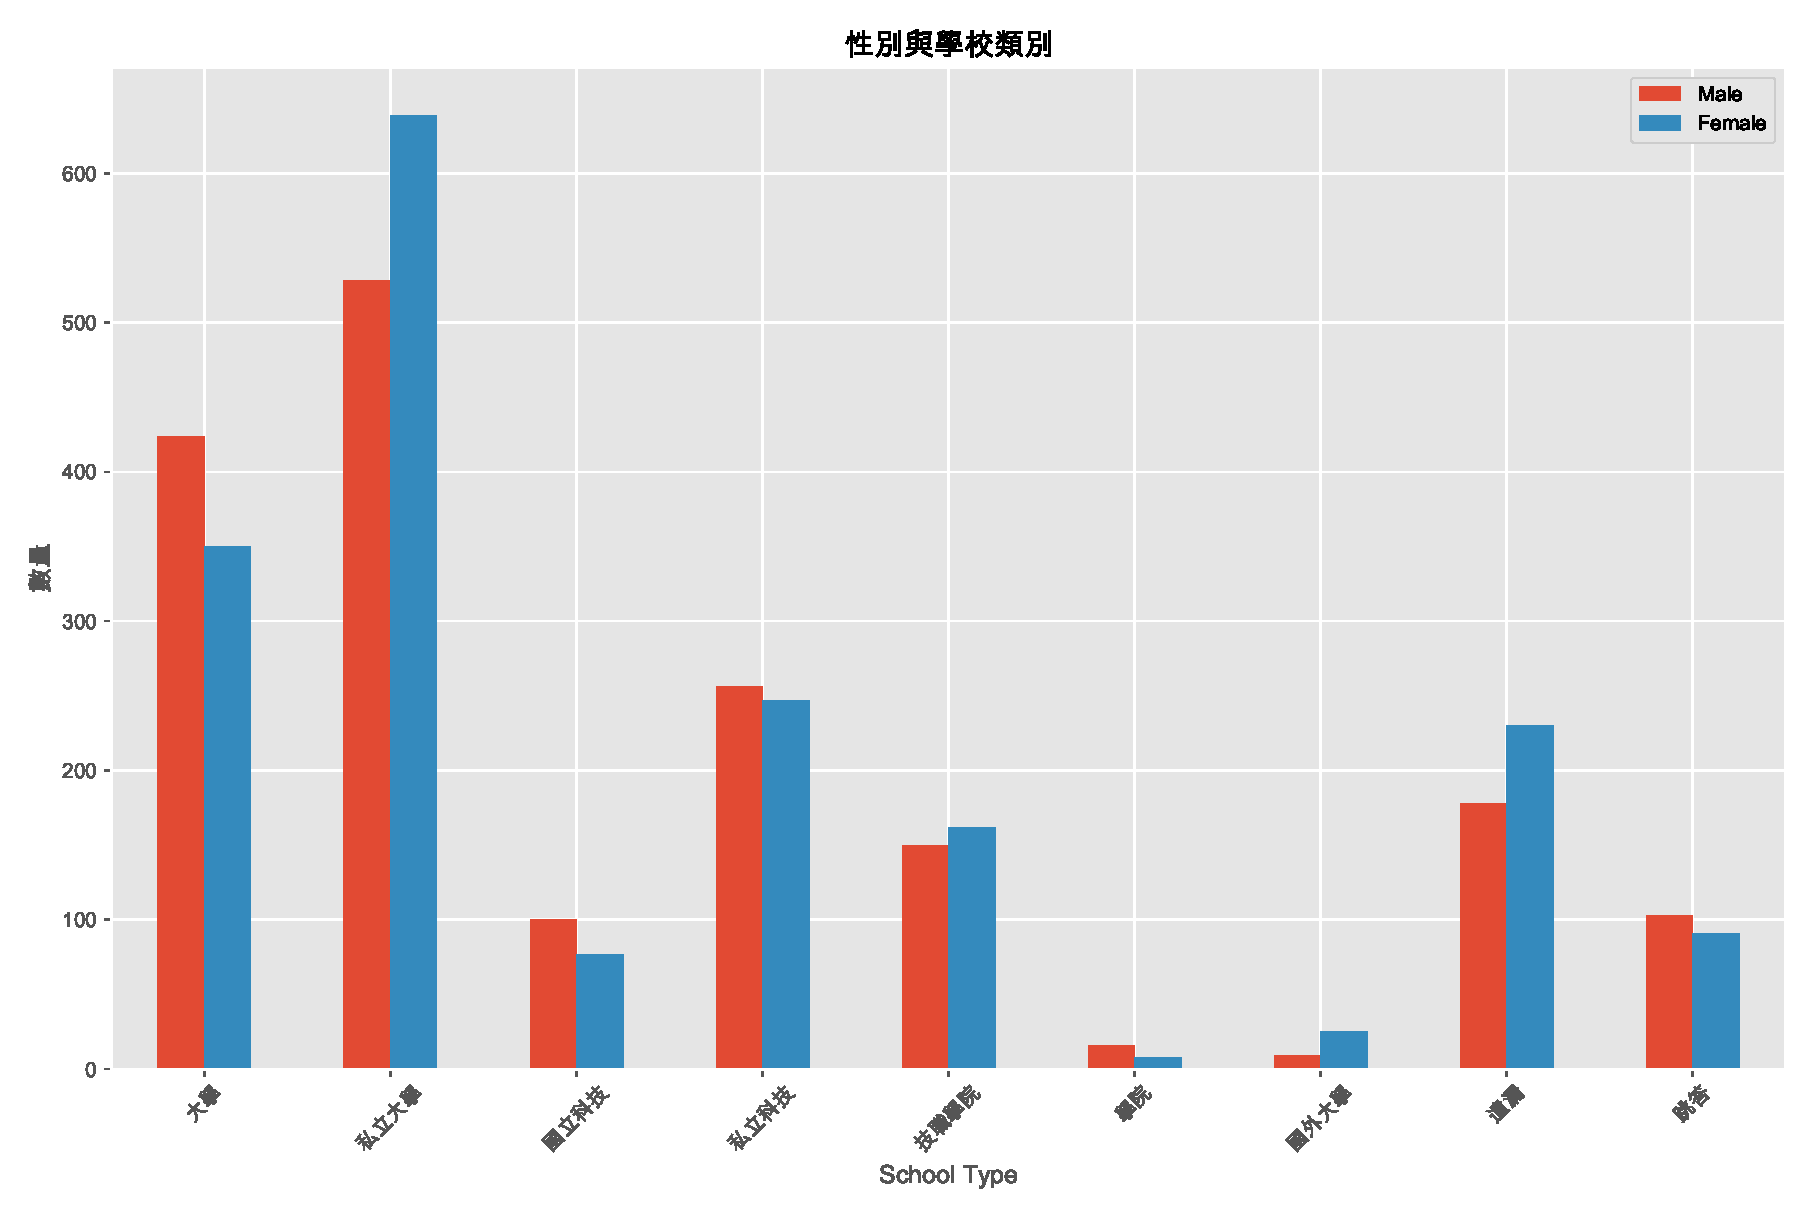
\includegraphics[width=0.8\linewidth]{\imgdir/gender_school.eps}
        \caption{學校種類與性別}
        \label{pic:shcool_gender}
\end{figure}

\begin{figure}[h]
    \centering    
        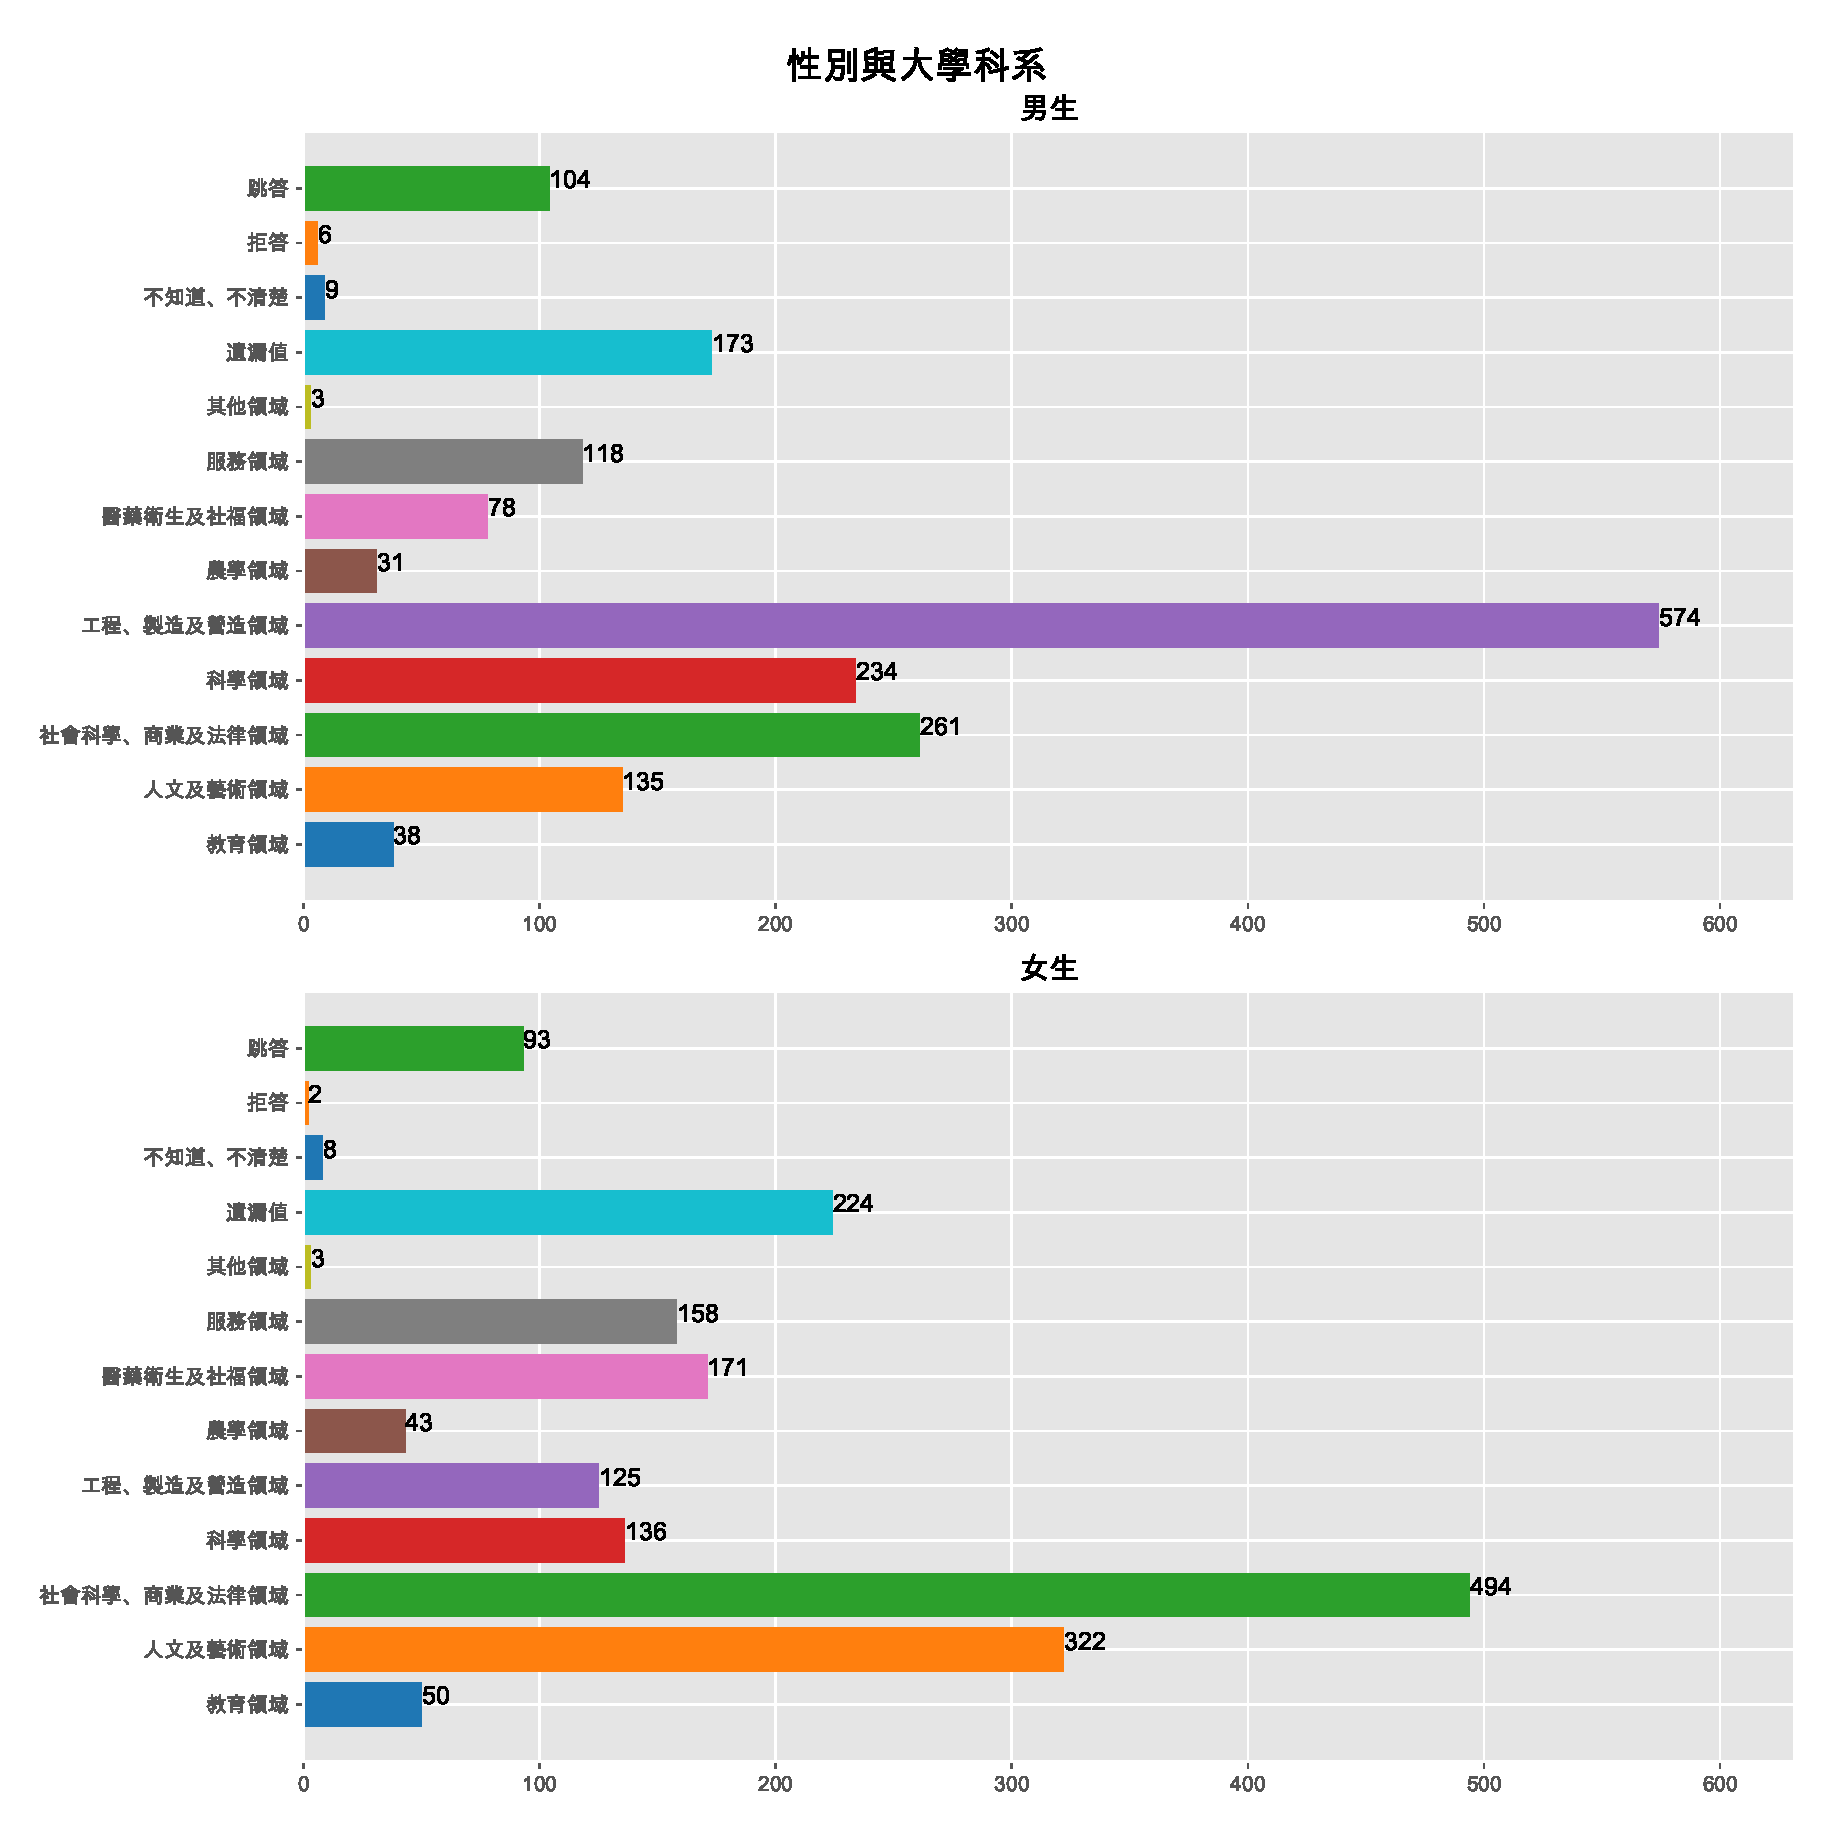
\includegraphics[width=0.8\linewidth]{\imgdir/gender_major.eps}
        \caption{大學科科系與性別}
        \label{pic:major_gender}
\end{figure}




%%%%%%%%%%%%%%%
\clearpage
\subsubsection{學校進入職場}

從學校步入職場的分析,多數受訪於目前是否有工作、是否為第一份工作,答覆上較多資料缺失。因此在表 \ref{tab:exper_curret} 、 \ref{tab:exper_first} 較多為缺失,值得注意為受者答覆2-3幾年的工作經驗,為首次調查中最為多數,其二為私立性質院校,較多受訪者答覆有工作經驗。目前工作經驗的計算有不同,根據原始受訪問卷中問及受訪者,第一份工作和現在的工作,受訪者可能因種種因素,目前所做的工作非最初工作,約有101位答覆,工作有轉換。計算工作經驗部分暫且以兩種方是呈現。



\begin{table}[ht]
\centering
\renewcommand{\arraystretch}{1.3} %%% Adjust the row height
\extrarowheight=5pt
\caption{工作經驗(目前工作計算)}
\begin{adjustbox}{width=\textwidth}
\begin{tabular}{l*{7}{c}}
\toprule
& \multicolumn{7}{c}{工作經驗(目前工作計算)} \\
\cmidrule(lr){2-8}
\multirow{2}{*}{大學學校種類} & \multirow{2}{*}{4年-5年} & \multirow{2}{*}{3年-4年} & \multirow{2}{*}{2年-3年} & \multirow{2}{*}{1年-2年} & \multirow{2}{*}{1年內} & \multirow{2}{*}{遺漏、跳答} & \multirow{2}{*}{Total} \\
&  &  & &  & &、不清楚、跳答 &  \\
\midrule
國立大學 & 0 & 1 & 4 & 1 & 2 & 766 & 774 \\
私立大學 & 1 & 4 & 9 & 17 & 16 & 1,120 & 1,167 \\
國立科技大學 & 0 & 0 & 6 & 2 & 5 & 164 & 177 \\
私立科技大學 & 0 & 1 & 29 & 18 & 27 & 428 & 503 \\
技職學院、專科學校 & 0 & 0 & 20 & 17 & 24 & 251 & 312 \\
學院 & 0 & 0 & 0 & 1 & 0 & 23 & 24 \\
國外大學、其他 & 0 & 0 & 0 & 0 & 0 & 34 & 34 \\
遺漏、不清楚、拒答 & 0 & 0 & 1 & 0 & 1 & 406 & 408 \\
跳答 & 0 & 2 & 53 & 40 & 44 & 55 & 194 \\
Total & 1 & 8 & 122 & 96 & 119 & 3,247 & 3,593 \\
\bottomrule
\label{tab:exper_curret}
\end{tabular}
\end{adjustbox}
\end{table}

\begin{table}[H]
\centering
\renewcommand{\arraystretch}{1.3} %%%把表格的高拉大
\extrarowheight=4pt
\caption{工作經驗(第一份工作計算)}
\begin{adjustbox}{width=\textwidth}
\begin{tabular}{l*{8}{c}}
\toprule
& \multicolumn{8}{c}{工作經驗(第一份工作計算)} \\
\cmidrule(lr){2-9}
\multirow{2}{*}{大學學校種類} & \multirow{2}{*}{5年} & \multirow{2}{*}{4年-5年} & \multirow{2}{*}{3年-4年} & \multirow{2}{*}{2年-3年} & \multirow{2}{*}{1年-2年} & \multirow{2}{*}{1年內} & \multirow{2}{*}{遺漏、跳答} & \multirow{2}{*}{Total} \\
& & & & & & &、不清楚、跳答 & \\
\midrule
國立大學 & 0 & 0 & 1 & 0 & 0 & 0 & 773 & 774 \\
私立大學 & 1 & 1 & 0 & 5 & 8 & 0 & 1,152 & 1,167 \\
國立科技大學 & 0 & 0 & 0 & 0 & 1 & 0 & 176 & 177 \\
私立科技大學 & 1 & 1 & 1 & 15 & 3 & 2 & 480 & 503 \\
技職學院、專科學校 & 0 & 0 & 2 & 9 & 5 & 0 & 296 & 312 \\
學院 & 0 & 0 & 0 & 0 & 0 & 0 & 24 & 24 \\
國外大學、其他 & 0 & 0 & 0 & 0 & 0 & 0 & 34 & 34 \\
遺漏、不清楚、拒答 & 0 & 0 & 0 & 0 & 0 & 0 & 408 & 408 \\
跳答 & 0 & 0 & 3 & 25 & 4 & 3 & 159 & 194 \\
Total & 2 & 2 & 7 & 54 & 21 & 5 & 3,502 & 3,593 \\
\bottomrule
\label{tab:exper_first}
\end{tabular}
\end{adjustbox}
\end{table}


%%%%%%%%%%%%%%%%%

薪酬與學歷情況,透過
\begin{table}[ht]
\centering
\renewcommand{\arraystretch}{1.3} %%%把表格的高拉大
\extrarowheight=4pt
\caption{大學學校種類與薪酬}
\begin{adjustbox}{width=\textwidth}
\begin{tabular}{l*{8}{c}}
\toprule
& \multicolumn{8}{c}{薪酬經過重新分組} \\
\cmidrule(lr){2-9}
大學學校種類 & 2萬以下 & 2萬以上& 3萬以上 & 4萬以上 & 5萬以上 & 遺漏、 & 跳答 & Total \\
		   &    &-3萬以下    & -4萬以下  &- 5萬以下    & -6萬以下   & 不清楚、拒答   &   &  \\
\midrule
國立大學 & 5 & 3 & 0 & 0 & 0 & 3 & 763 & 774 \\
私立大學 & 28 & 17 & 2 & 0 & 0 & 2 & 1,118 & 1,167 \\
國立科技大學 & 7 & 6 & 0 & 0 & 0 & 1 & 163 & 177 \\
私立科技大學 & 46 & 24 & 4 & 0 & 0 & 6 & 423 & 503 \\
技職學院、專科學校 & 27 & 27 & 4 & 0 & 1 & 3 & 250 & 312 \\
學院 & 0 & 1 & 0 & 0 & 0 & 0 & 23 & 24 \\
國外大學、其他 & 0 & 0 & 0 & 0 & 0 & 0 & 34 & 34 \\
遺漏、不清楚、拒答 & 1 & 1 & 0 & 0 & 0 & 395 & 11 & 408 \\
跳答 & 37 & 62 & 23 & 3 & 1 & 18 & 50 & 194 \\
Total & 151 & 141 & 33 & 3 & 2 & 428 & 2,835 & 3,593 \\
\bottomrule
\label{tab:school_wage}
\end{tabular}
\end{adjustbox}
\end{table}



\begin{figure}[H]
    \centering    
        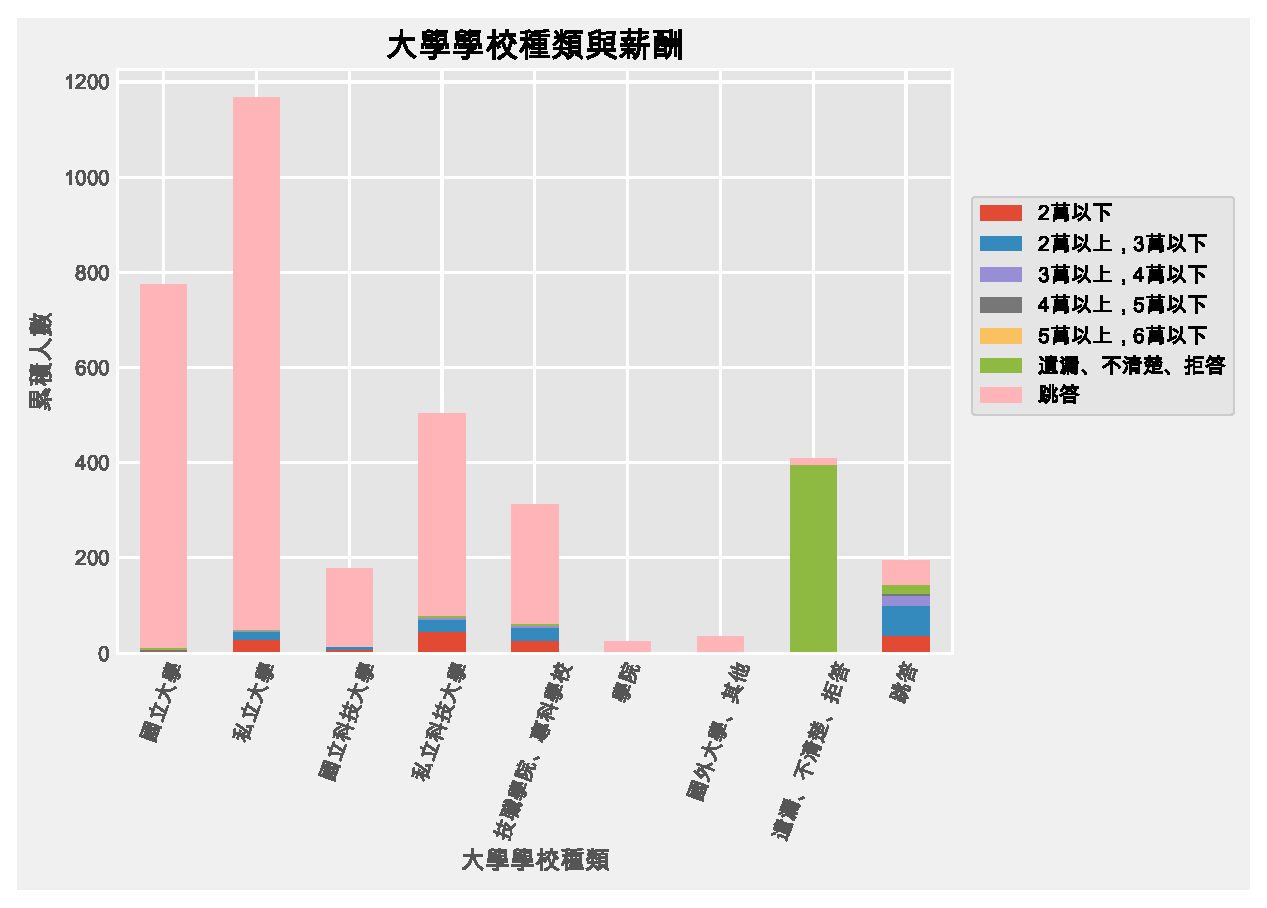
\includegraphics[width=0.9\linewidth]{\imgdir/school_type_salary.eps}
        \caption{學校種類與薪酬}
        \label{pic:school_salary}
\end{figure}



\begin{table}[ht]
\centering
\caption{變數之間的相關係數}
\begin{tabular}{lcccccc}
\toprule
& \textbf{salary\_modfy} & \textbf{gender} & \textbf{school} & \textbf{major} & \textbf{exper\_cur} & \textbf{exper} \\
\midrule
\textbf{salary\_modfy} & 1.0000 & - & - & - & - & - \\
\textbf{gender} & -0.0022 & 1.0000 & - & - & - & - \\
\textbf{school} & -0.3772 & 0.0272 & 1.0000 & - & - & - \\
\textbf{major} & -0.3187 & 0.0119 & 0.8437 & 1.0000 & - & - \\
\textbf{exper\_cur} & 0.8644 & 0.0187 & -0.2727 & -0.2004 & 1.0000 & - \\
\textbf{exper} & 0.4685 & -0.0239 & -0.1323 & -0.0925 & 0.3327 & 1.0000 \\
\bottomrule
\end{tabular}
\end{table}



%%%%%%%%%%%%%%%%%%%%

\section{2013年度調查-電訪}

















\end{document}
